\documentclass{standalone}
\usepackage{tikz}
\usetikzlibrary{patterns, positioning}


\begin{document}
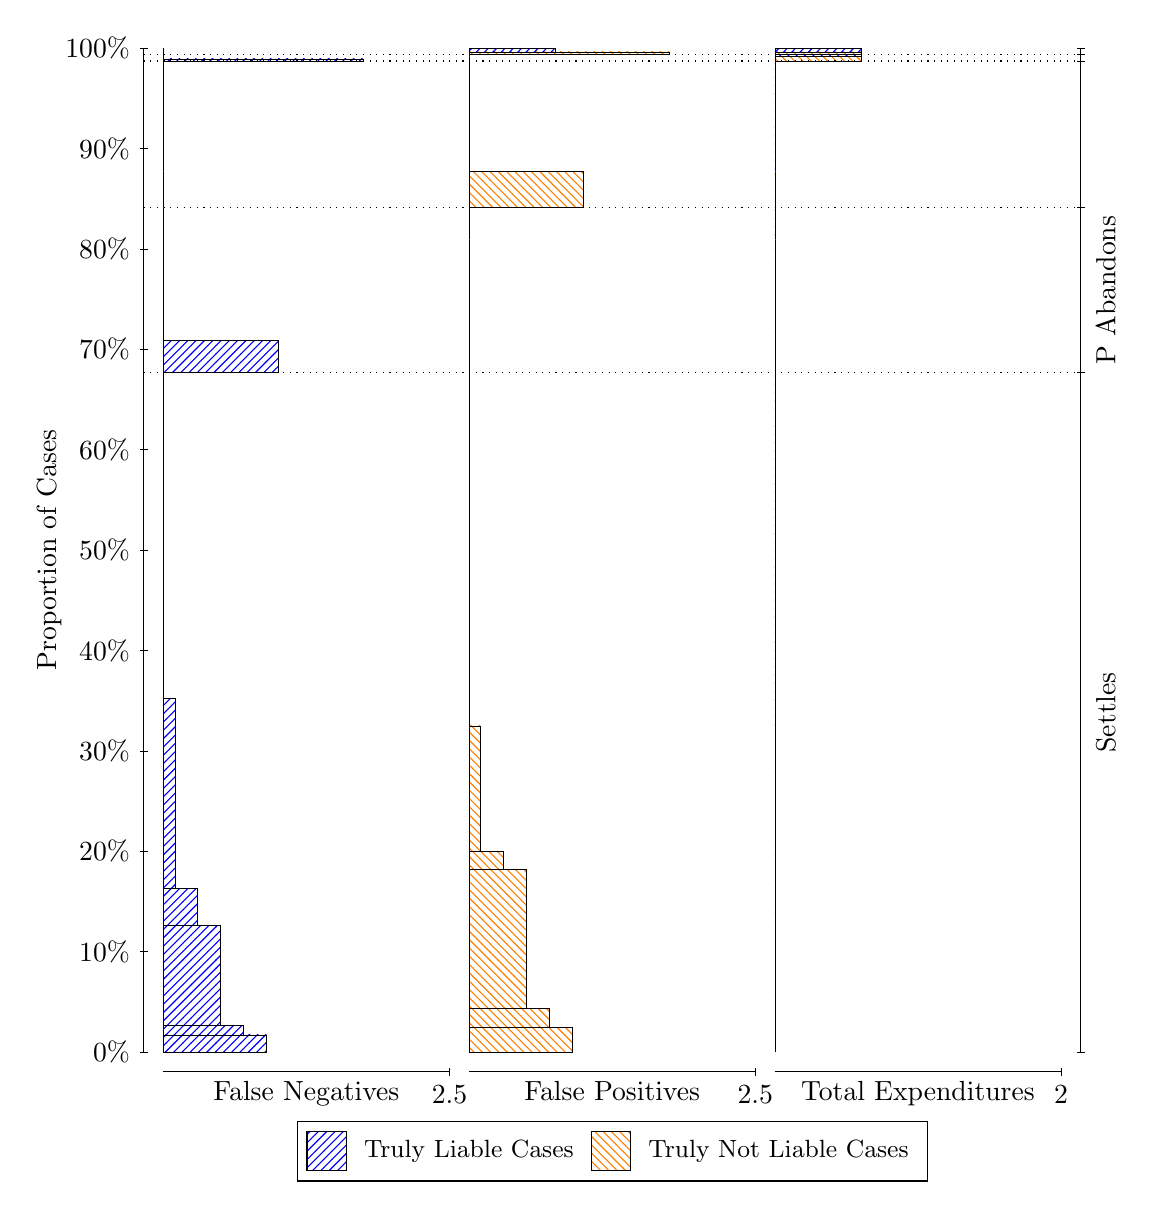
\begin{tikzpicture}
\draw[black, very thin] (1.5,1.75) -- (1.5,14.5);
\node[rotate=90, text=black, anchor=center] at (0.3, 8.125) {Proportion of Cases};
\draw[black, very thin] (1.45,1.75) -- (1.55,1.75);
\node[text=black, anchor=east] at (1.45, 1.75) {0\%};
\draw[black, very thin] (1.45,3.025) -- (1.55,3.025);
\node[text=black, anchor=east] at (1.45, 3.025) {10\%};
\draw[black, very thin] (1.45,4.3) -- (1.55,4.3);
\node[text=black, anchor=east] at (1.45, 4.3) {20\%};
\draw[black, very thin] (1.45,5.575) -- (1.55,5.575);
\node[text=black, anchor=east] at (1.45, 5.575) {30\%};
\draw[black, very thin] (1.45,6.85) -- (1.55,6.85);
\node[text=black, anchor=east] at (1.45, 6.85) {40\%};
\draw[black, very thin] (1.45,8.125) -- (1.55,8.125);
\node[text=black, anchor=east] at (1.45, 8.125) {50\%};
\draw[black, very thin] (1.45,9.4) -- (1.55,9.4);
\node[text=black, anchor=east] at (1.45, 9.4) {60\%};
\draw[black, very thin] (1.45,10.675) -- (1.55,10.675);
\node[text=black, anchor=east] at (1.45, 10.675) {70\%};
\draw[black, very thin] (1.45,11.95) -- (1.55,11.95);
\node[text=black, anchor=east] at (1.45, 11.95) {80\%};
\draw[black, very thin] (1.45,13.225) -- (1.55,13.225);
\node[text=black, anchor=east] at (1.45, 13.225) {90\%};
\draw[black, very thin] (1.45,14.5) -- (1.55,14.5);
\node[text=black, anchor=east] at (1.45, 14.5) {100\%};

\draw[black, very thin] (13.4,1.75) -- (13.4,14.5);
\draw[black, very thin] (13.35,1.75) -- (13.45,1.75);
\node[anchor=west] at (13.35, 1.75) {};
\draw[black, very thin] (13.35,10.377) -- (13.45,10.377);
\node[anchor=west] at (13.35, 10.377) {};
\draw[black, very thin] (13.35,12.474) -- (13.45,12.474);
\node[anchor=west] at (13.35, 12.474) {};
\draw[black, very thin] (13.35,14.335) -- (13.45,14.335);
\node[anchor=west] at (13.35, 14.335) {};
\draw[black, very thin] (13.35,14.422) -- (13.45,14.422);
\node[anchor=west] at (13.35, 14.422) {};
\draw[black, very thin] (13.35,14.5) -- (13.45,14.5);
\node[anchor=west] at (13.35, 14.5) {};

\draw[black, very thin, pattern color=blue, pattern=north east lines] (1.75,1.75) rectangle (3.058,1.9663);
\draw[black, very thin, pattern color=blue, pattern=north east lines] (1.75,1.9663) rectangle (2.7673,2.0878);
\draw[black, very thin, pattern color=blue, pattern=north east lines] (1.75,2.0878) rectangle (2.4767,3.3596);
\draw[black, very thin, pattern color=blue, pattern=north east lines] (1.75,3.3596) rectangle (2.186,3.8306);
\draw[black, very thin, pattern color=blue, pattern=north east lines] (1.75,3.8306) rectangle (1.8953,6.236);
\draw[black, very thin, pattern color=orange, pattern=north west lines] (1.75,6.236) rectangle (1.75,10.377);
\draw[black, very thin, pattern color=blue, pattern=north east lines] (1.75,10.377) rectangle (3.2033,10.783);
\draw[black, very thin, pattern color=orange, pattern=north west lines] (1.75,10.783) rectangle (1.75,12.474);
\draw[black, very thin, pattern color=orange, pattern=north west lines] (1.75,12.474) rectangle (1.75,12.931);
\draw[black, very thin, pattern color=blue, pattern=north east lines] (1.75,12.931) rectangle (1.75,14.335);
\draw[black, very thin, pattern color=blue, pattern=north east lines] (1.75,14.335) rectangle (4.2933,14.363);
\draw[black, very thin, pattern color=orange, pattern=north west lines] (1.75,14.363) rectangle (1.75,14.422);
\draw[black, very thin, pattern color=orange, pattern=north west lines] (1.75,14.422) rectangle (1.75,14.45);
\draw[black, very thin, pattern color=blue, pattern=north east lines] (1.75,14.45) rectangle (1.75,14.5);
\draw[black, very thin, pattern color=orange, pattern=north west lines] (5.6333,1.75) rectangle (6.9413,2.0635);
\draw[black, very thin, pattern color=orange, pattern=north west lines] (5.6333,2.0635) rectangle (6.6507,2.3064);
\draw[black, very thin, pattern color=orange, pattern=north west lines] (5.6333,2.3064) rectangle (6.36,4.0657);
\draw[black, very thin, pattern color=orange, pattern=north west lines] (5.6333,4.0657) rectangle (6.0693,4.3012);
\draw[black, very thin, pattern color=orange, pattern=north west lines] (5.6333,4.3012) rectangle (5.7787,5.8907);
\draw[black, very thin, pattern color=blue, pattern=north east lines] (5.6333,5.8907) rectangle (5.6333,10.377);
\draw[black, very thin, pattern color=orange, pattern=north west lines] (5.6333,10.377) rectangle (5.6333,12.068);
\draw[black, very thin, pattern color=blue, pattern=north east lines] (5.6333,12.068) rectangle (5.6333,12.474);
\draw[black, very thin, pattern color=orange, pattern=north west lines] (5.6333,12.474) rectangle (7.0867,12.931);
\draw[black, very thin, pattern color=blue, pattern=north east lines] (5.6333,12.931) rectangle (5.6333,14.335);
\draw[black, very thin, pattern color=orange, pattern=north west lines] (5.6333,14.335) rectangle (5.6333,14.394);
\draw[black, very thin, pattern color=blue, pattern=north east lines] (5.6333,14.394) rectangle (5.6333,14.422);
\draw[black, very thin, pattern color=orange, pattern=north west lines] (5.6333,14.422) rectangle (8.1767,14.45);
\draw[black, very thin, pattern color=blue, pattern=north east lines] (5.6333,14.45) rectangle (6.7233,14.5);
\draw[black, very thin, pattern color=orange, pattern=north west lines] (9.5167,1.75) rectangle (9.5167,5.8907);
\draw[black, very thin, pattern color=blue, pattern=north east lines] (9.5167,5.8907) rectangle (9.5167,10.377);
\draw[black, very thin, pattern color=orange, pattern=north west lines] (9.5167,10.377) rectangle (9.5167,12.068);
\draw[black, very thin, pattern color=blue, pattern=north east lines] (9.5167,12.068) rectangle (9.5167,12.474);
\draw[black, very thin, pattern color=orange, pattern=north west lines] (9.5167,12.474) rectangle (9.5167,12.931);
\draw[black, very thin, pattern color=blue, pattern=north east lines] (9.5167,12.931) rectangle (9.5167,14.335);
\draw[black, very thin, pattern color=orange, pattern=north west lines] (9.5167,14.335) rectangle (10.607,14.394);
\draw[black, very thin, pattern color=blue, pattern=north east lines] (9.5167,14.394) rectangle (10.607,14.422);
\draw[black, very thin, pattern color=orange, pattern=north west lines] (9.5167,14.422) rectangle (10.607,14.45);
\draw[black, very thin, pattern color=blue, pattern=north east lines] (9.5167,14.45) rectangle (10.607,14.5);
\draw[black, dotted] (1.5,10.377) -- (13.4,10.377);
\draw[black, dotted] (1.5,12.474) -- (13.4,12.474);
\draw[black, dotted] (1.5,14.335) -- (13.4,14.335);
\draw[black, dotted] (1.5,14.422) -- (13.4,14.422);
\draw[black, very thin] (1.75,1.5) -- (5.3833,1.5);
\node[text=black, anchor=north] at (3.5667, 1.5) {False Negatives};
\draw[black, very thin] (5.3833,1.45) -- (5.3833,1.55);
\node[text=black, anchor=north] at (5.3833, 1.45) {2.5};

\draw[black, very thin] (5.6333,1.5) -- (9.2667,1.5);
\node[text=black, anchor=north] at (7.45, 1.5) {False Positives};
\draw[black, very thin] (9.2667,1.45) -- (9.2667,1.55);
\node[text=black, anchor=north] at (9.2667, 1.45) {2.5};

\draw[black, very thin] (9.5167,1.5) -- (13.15,1.5);
\node[text=black, anchor=north] at (11.333, 1.5) {Total Expenditures};
\draw[black, very thin] (13.15,1.45) -- (13.15,1.55);
\node[text=black, anchor=north] at (13.15, 1.45) {2};

\node[text=black, centered, rotate=90] at (13.72, 6.0633) {Settles};
\node[text=black, centered, rotate=90] at (13.72, 11.425) {P Abandons};




\draw (7.449999999999999,1.5) node[draw=none] (baseCoordinate) {};
\begin{scope}[align=center]
        \matrix[scale=0.5, draw=black, below=0.5cm of baseCoordinate, nodes={draw}, column sep=0.1cm]{
            \node[rectangle, draw, minimum width=0.5cm, minimum height=0.5cm, pattern color=blue, pattern=north east lines] {}; &
            \node[draw=none, font=\small, text=black] (B) {Truly Liable Cases}; &
            \node[rectangle, draw, minimum width=0.5cm, minimum height=0.5cm, pattern color=orange, pattern=north west lines] {}; &
            \node[draw=none, font=\small, text=black] (B) {Truly Not Liable Cases}; \\
            };
\end{scope}

\end{tikzpicture}
\end{document}